% !TEX encoding = UTF-8 Unicode

\documentclass[a4paper]{article}

\usepackage{color}
\usepackage{url}
\usepackage[T2A]{fontenc} 
\usepackage[utf8]{inputenc}
\usepackage{graphicx}

\usepackage[english,serbianc]{babel}

\usepackage[unicode]{hyperref}
\hypersetup{colorlinks,citecolor=green,filecolor=green,linkcolor=blue,urlcolor=blue}


\newtheorem{primer}{Пример}[section]


\begin{document}

\title{Нигеријска превара\\ \small{Семинарски рад у оквиру курса\\Рачунарство и друштво\\ Математички факултет}}

\author{Павле Савић\\ pavlesavic1389@gmail.com}
\date{10.~август 2021.}
\maketitle

\abstract{
Превара 419 (такође позната и као нигеријска превара) је популаран облик преваре у којем преварант превари жртву да плати одређену суму новца под обећањем будуће, веће исплате. У овом раду обрадићемо начине организације ове преваре и како су они еволуирали кроз време, ослањајући се на рад француских истраживача са \emph{Eurocom}-а \cite{article}. Посебно говоримо о улози телефонских бројева као важних идентификатора за груписање порука и приказујемо начин на који преваранти воде своје кампање. Заправо, пошто жртва мора ступити у контакт са скамером, адреса е-поште и телефонски бројеви морају бити аутентични, ретко се мењају и користе се током дужег временског периода.
}

\tableofcontents

\newpage

\section{Увод}
\label{sec:uvod}
Нигеријска превара \cite{def} (превара 419) односи се на одељак 419 у нигеријском кривичном законику. Овај проблем познат је већ неколико деценија. Назив обухвата многе варијације ове врсте превара, попут превара са авансним провизијама, лажне лутрије, преваре са црним новцем итд. Првобитно је феномен преваре 419 започео путем поште, а затим се развио у посао који се прво водио путем факса, а касније путем е-поште. Кривично гоњење за такве криминалне активности је компликовано \cite{prosecuting} и нападачи га често могу избећи. Због тога се извештаји о таквим илегалним радњама и даље појављују на друштевним мрежама и онлајн заједницама, нпр. сајт \emph{419scam.org} \cite{org} постоји како би се умањио ризик и помогло корисницима да идентификују преваре.

Данас, овај тип преваре често се сматра типом нежељене поште (енг.~{\em spam}). Међутим, док се највећи део нежељене поште у новије време масовно шаље аутоматски коришћењем ботнета, нигеријска превара се и даље у великој мери обавља ручно. \emph{Спамери} своје жртве нападају инжењерским напорима, док се \emph{скамери} ослањају на људске факторе: сажаљење, похлепу и технике друштвеног инжењеринга користећи примитивније алате. Посебна карактеристика превара путем е-поште је комуникациони канал постављен да допре до жртве: \emph{скамери} чешће користе е-пошту и/или телефонске бројеве \cite{phone} док је за друге облике \emph{спама} вероватније да прослеђују своје жртве на контаминиране УРЛ-адресе. На пример, студија о \emph{спам} кампањама из 2009. године \cite{study} показује да 59\% нежељене поште садржи УРЛ (\emph{скам} је посматран као подскуп \emph{спама}). Међутим, и поред огромне количине аутоматски генерисане нежељене поште, 419 \emph{скам} поруке и даље представљају сталан проблем који узрокује значајне личне финансијске губитке за бројне жртве широм света.

Традиционални \emph{спам} и \emph{скам} сценарији (не 419) темељно су проучени (нпр. \cite{study,cishi}), већина техника ове природе ослања се на огромне количине сличних порука. Насупрот томе, 419 поруке вероватније ће бити послате у мањем броју копија и са налога веб поште. На тај начин, нападачи имају за циљ да остану неопажени од стране традиционалних филтера за нежељену пошту и избегну скретање пажње на злоупотребљене налоге веб поште. Прецизне методе дистрибуције 419 \emph{скам} порука нису проучаване тако детаљно као, на пример, дистрибуција \emph{спам} поште путем \emph{ботнета}. На основу {\em Microsoft Security Intelligence Reports} \cite{microsoft}, 419 поруке чиниле су у просеку 8\% нежељене е-поште у периоду 2009-2014.

Студија из 2013. године \cite{phone} описује употребу телефонских бројева у бројним злонамерним активностима. Аутори су показали да су телефонски бројеви које користе \emph{скамери} често активни током дужег временског периода и да се често користе изнова и изнова у различитим мејловима, што их чини потенцијално атрактивном метом за повезивање \emph{скам} порука и идентификацију преваре. Ову хипотезу подробније ћемо тестирати користећи телефонске бројеве и друге функције е-поште за аутоматско откривање и проучавање \emph{скам} кампањи коришћењем јавног скупа података.

Наш циљ је да проучимо како \emph{скамери} организују своје преваре, гледајући међусобне везе између налога е-поште, телефонских бројева и тема е-поште које користе. У ту сврху користи се алгоритам одлучивања са више критеријума за ефикасно \emph{кластеровање} (груписање) \emph{скам} порука које деле минималан број заједничких особина, чак и у присуству променљивих (енг.~{\em volatile}) особина. Због овог скупа заједничких карактеристика, \emph{скам} мејлови који потичу од истих нападача вероватно ће бити груписани заједно, што нам омогућава да стекнемо увид у \emph{скам} кампању. Поред тога, оцењујемо квалитет и доследност наших резултата груписања. Ради тога вршимо анализу прага осетљивости, као и процену хомогености кластера користећи компактност графикона и енг.~{\em Adjusted Rand Index} као метрике.

У анализи приказаној у обрађеном раду \cite{article} идентификовано је преко 1000 различитих превара, и за већину њих, телефонски бројеви представљају камен темељац који је омогућио повезивање различитих делова. На овај начин откривене су и неке кампање већег обима (енг.~{\em macro-cluster}), сачињене од међусобно слабо повезаних \emph{скам кластера} који одражавају различите операције истих превараната. То се може приписати различитим \emph{скамовима} које организују исте криминалне групе, јер проналазимо исте телефонске бројеве или налоге е-поште који се поновно користе у различитим подкампањама.

Експериментално је утврђено да се ове методе могу искористити за проактивно идентификовање нових превара (или варијанти претходних) брзим повезивањем нове преваре са текућим кампањама, што би могло олакшати рад правним институцијама приликом кривичног гоњења превараната. Овај приступ се такође може искористити и за побољшање истрага других шема сајбера криминала евидентирањем и истраживањем различитих група сајбер криминалаца на основу њихових активности на мрежи. Употребљивост ове методологије је већ показана у контексту других безбедносних истрага, као што су анализе \emph{спам} поште дистрибуиране путем \emph{ботнета} \cite{botnet}, циљаних напада \cite{target} и лажних антивируса \cite{rogueav}.


\section{Скуп података}
У овом одељку описујемо скуп података коришћен за анализу 419 превара и пружамо неке статистичке податке о тим кампањама. Постоје различити извори превара које корисници често пријављују које потом сакупљају наменске заједнице, форуми и друге онлајн групе. Подаци одабрани за анализу су прикупљени са \emph{419scam.org - a 419 scam aggregator} јер овај сајт пружа обиман скуп унапред претпроцесираних података: заглавља, тела е-поште и неке већ издвојене атрибуте е-поште, попут категорије \emph{скама} и телефонских бројева. Важно је нагласити да подаци о IP-aдресама недостају. Анализирана је пошта за период од јануара 2009. до августа 2012. године.

У овој студији такође је искоришћена чињеница да телефонски бројеви могу означавати географску локацију, обично земљу у којој је телефон регистрован. Иако то не доказује са сигурношћу порекло поруке или \emph{скамера}, ипак реферише на земљу где се превара спроводи, а такође и повећава поверење жртве у примљену поруку. На пример, примање партнерске понуде из Уједињеног Краљевства могло би изгледати сумњиво ако телефонски контакт има нигеријски префикс или обавештење о лутрији са контакт подацима из афричке земље, док је жртва из Европе. Штавише, као што је показано у студији \cite{phone} бројеви мобилних телефона коришћених за нигеријску превару прецизно указују на државу пребивалишта власника телефона (нападача) јер је пронађено неколико случајева роминга. Због тога је атрибут телефонског броја довољно прецизан да означи географско порекло напада.

Добијени скуп података састоји се од 36.761 порука са 11.768 јединствених телефонских бројева. Опште статистике података приказане су у табели \ref{tab:tabela}. Прво што треба приметити је да је број адреса е-поште три пута већи од броја телефонских бројева, што указује на могућност набавке поштанских сандучића у злонамерне сврхе. Међутим, однос је и даље прилично низак, што указује на прилично јефтин и лак приступ телефонским бројевима. Још једна специфичност овог скупа података је да свака порука може садржати неколико адреса е-поште и телефонских бројева, при чему број различитих адреса е-поште може бити чак 5 по поруци: \emph{from} адреса,\emph{reply} адреса и друге адресе наведене у тексту поруке. Дакле, иако је прикупљено 36.761 порука, из њих је извучено 112.961 адреса е-поште.

\begin{table}[h!]
\begin{center}
\caption{Опште статистике}
\begin{tabular}{|c|c|} \hline
\textbf{Опис} & \textbf{Број} \\ \hline
Скам поруке & 36.761 \\ \hline
Јединствене поруке & 26.250\\ \hline
Укупно мејл адреса & 112.961\\ \hline
Јединствене мејл адресе & 34.723\\ \hline
Укупно телефонских бројева & 41.320\\ \hline
Јединствени телефонски бројеви & 11.768\\ \hline
Број држава & 12\\ \hline
\end{tabular}
\label{tab:tabela}
\end{center}
\end{table}

У обрађеном скупу података нису примећени значајнији налети \emph{скам} порука током трогодишњег периода (на месечном нивоу), што указује на то да су се поруке е-поште константно дистрибуирале током времена. Такође је важно напоменути да је скуп података углавном ограничен на европске и афричке регионе (са само неколико азијских узорака), што је последица начина на који власници вебсајтова прикупљају и класификују податке. Ипак, географска распрострањеност поменутих континената одражава се и на посматрани скуп података, искључујући малобројне изузетке.

Ради бољег разумевања скупа података, треба погледати време током којег су \emph{скамери} у \emph{скам} порукама користили мејл адресе и телефоне. 71\% адреса е-поште у овом скупу података коришћенo је само током једног дана. Преосталe су коришћенe у просеку по 79 дана. Телефонски бројеви имају дужи век трајања: 51\% коришћен је само 1 дан; остатак је коришћен у просеку 174 дана (око 6 месеци), што га чини важном особином приликом анализа засноване на \emph{кластеровању}.

Табела \ref{tab:tabela2} резимира географску дистрибуцију телефонских бројева. Бројеви из Уједињеног Краљевства двоструко су чешћи од нигеријских, и три пута чешћи од оних из Бенина, треће највеће групе. Холандија и Шпанија водеће су земље у Европи. УК треба сматрати посебним случајем. По извештајима \emph{419scam.org} и \cite{phone}, сви бројеви телефона из УК у овом скупу података припадају енг.~{\em personal numbering services} - сервисима који се користе за прослеђивање телефонских позива на друге телефонске бројеве и служе за маскирање стварне дестинације позиваоца. У посматраном скупу података постоји 44\% таквих телефонских бројева (сви са префиксом УК), још 44\% су бројеви мобилних телефона, 12\% су фиксне линије \cite{phone}, мање од 1\% телефона су непостојећи.

\begin{table}[h!]
\begin{center}
\caption{Телефони по државама}
\begin{tabular}{|c|c|c|} \hline
\textbf{Држава} & \textbf{Укупно телефона} & \textbf{Укупно (\%)}\\ \hline
Уједињено Краљевство & 4.499 & 43\\ \hline
Нигерија & 3.121 & 30\\ \hline
Бенин & 1.448 & 14\\ \hline
Јужна Африка & 562 & 5\\ \hline
Шпанија & 372 & 4\\ \hline
Холандија & 263 & 3\\ \hline
Обала Слоноваче & 89 & 1\\ \hline
Кина & 68 & 1\\ \hline
Сенегал & 47 & 0.5\\ \hline
Того & 11 & 0.1\\ \hline
Индонезија & 1 & 0.01\\ \hline
\end{tabular}
\label{tab:tabela2}
\end{center}
\end{table}

Порукама које су иницијално класификоване као превара 419 \emph{419scam.org} \cite{org} додељује и категорију. Око 64\% тих порука сврстано је у категорију \emph{'419 scam'} која је поткатегорија преваре 419 и односи се посебно на врсте финансијских превара, нпр. преваре са трансакцијама, изгубљена средства итд. Према извештају \cite{org} већина преосталих мејлова (24\%) припада поткатегорији \emph{'Fake lottery'}. Међутим, ова дистрибуција се временом мењала као што је приказано на слици \ref{fig:slika}. Посебно, велика разлика може се приметити између 2009. и 2011. када је \emph{'419 scam'} категорија постала доминантна. У августу 2012. било је 5 пута више \emph{'419 scam'} него \emph{'Fake lottery'} порука. То може бити последица застарелог процеса категоризације, јер се \emph{скам} може мењати и еволуирати временом. Из тог разлога, користи се процес аутоматског идентификовања врсте преваре који се заснива на фреквенцији речи у порукама. Такође примећујемо да је већина \emph{'Fake lottery'} превара повезана са европским телефонским бројевима што сугерише да се ова категорија шаље циљаној публици. Код \emph{'419 scam'} порука, нападачи користе готово подједнако често нигеријске и британске бројеве (слика \ref{fig:slika1}). Од 2011. значајнију улогу почиње да игра и Бенин.

\begin{figure}[h!]
\begin{center}
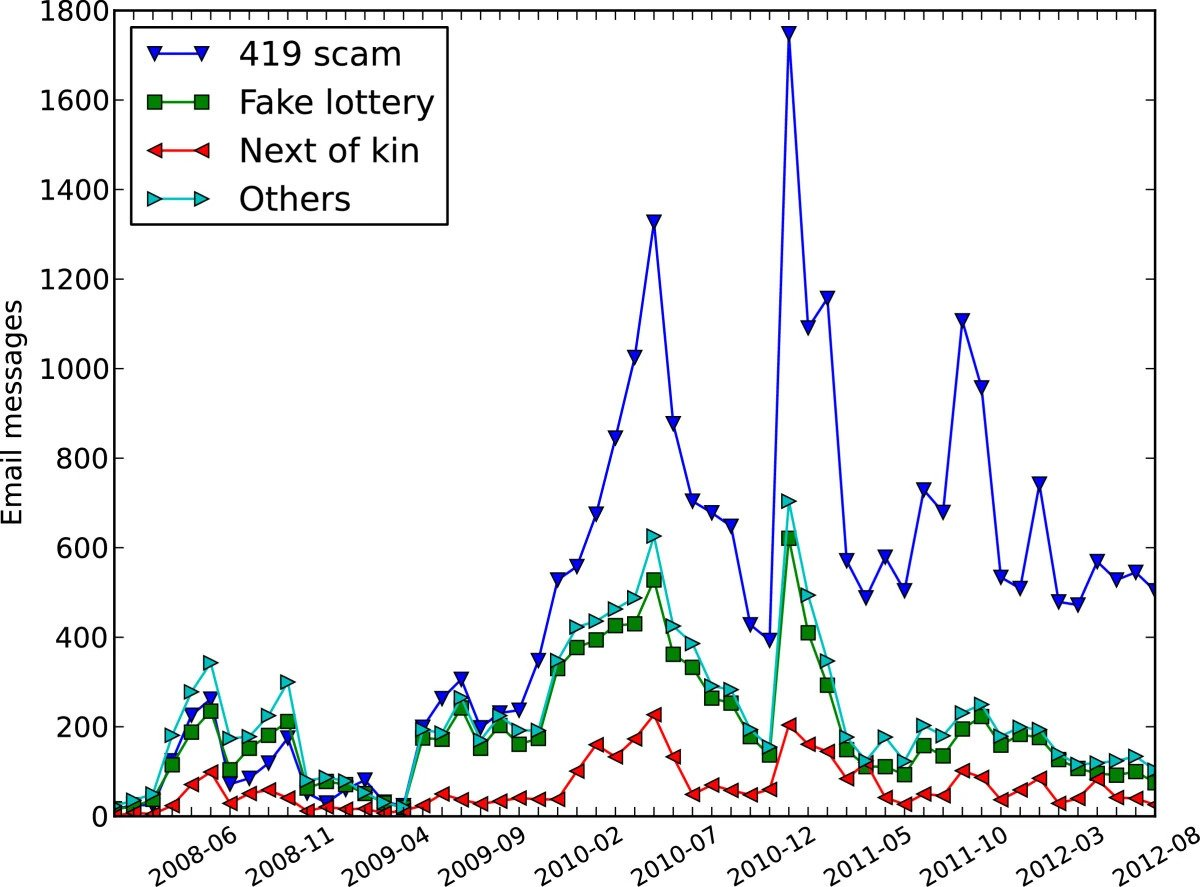
\includegraphics[scale=0.2]{slike/1.jpg}
\end{center}
\caption{Scam email categories over time}
\label{fig:slika}
\end{figure}

\begin{figure}[h!]
\begin{center}
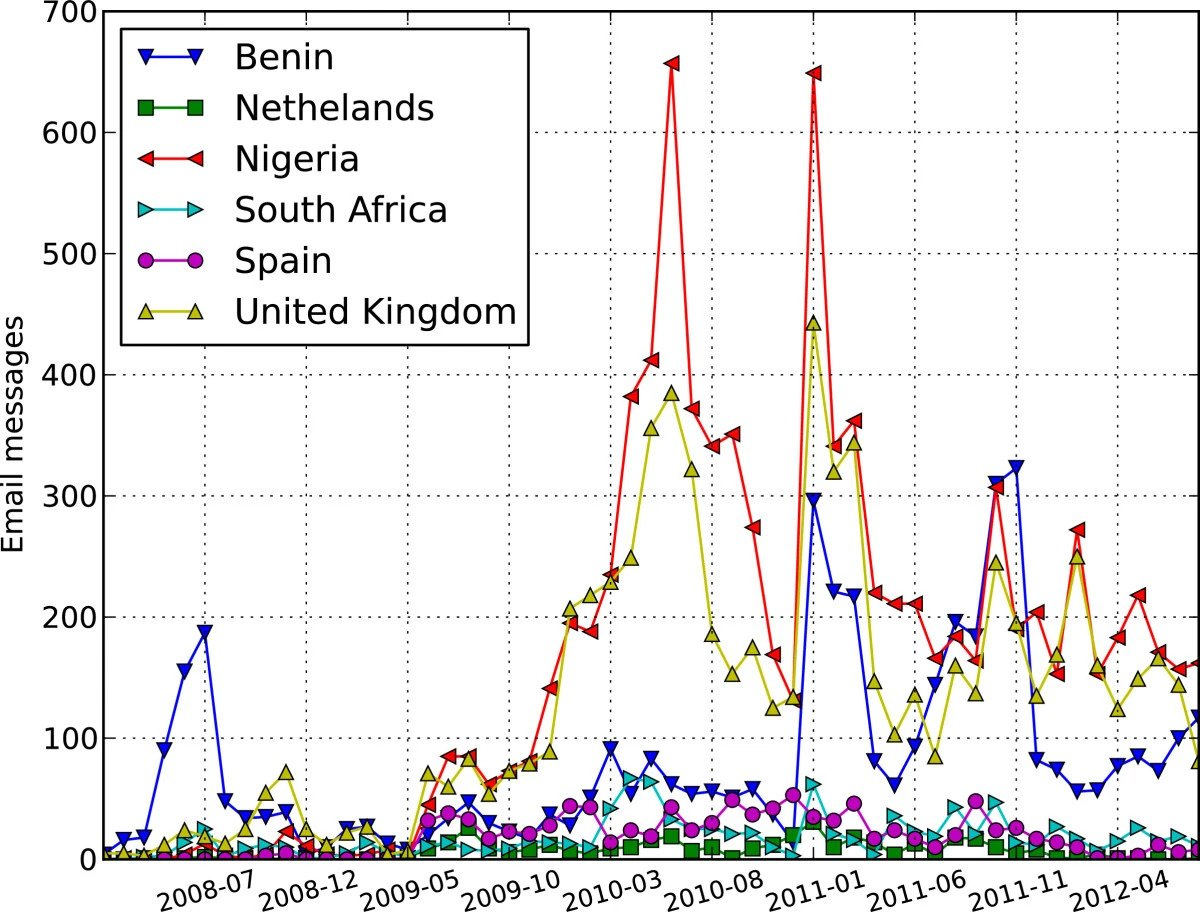
\includegraphics[scale=0.2]{slike/2.jpg}
\end{center}
\caption{‘419 scam’ category phone numbers over time by countries}
\label{fig:slika1}
\end{figure}

\section{Методе анализе података}
У овом одељку описујемо методе које се за користе за идентификовање група сличних 419 \emph{скам} порука за које се верује да су део истих кампања, а потом представљамо резултате. Користимо две различите метрике за процену квалитета и доследности креираних кластера (кампања). Коначно, из тела ових порука издвајамо кључне речи које се највише понављају како бисмо побољшали категоризацију.

\subsection{Кластеровање \emph{скам} порука : \emph{'TRIAGE'} приступ}
Да бисмо идентификовали групе \emph{скам} порука које имају изгледа да буду део кампање коју је организовала иста група људи, кластеровали смо све \emph{скам} поруке користећи \emph{'TRIAGE'} - \emph{framework} за безбедносно истраживање података који користи предности анализе више критеријума за груписање догађаја на основу подскупова заједничких елемената (касније названих особинама). Захваљујући овом приступу кластеровања по више критеријума, \emph{'TRIAGE'} идентификује сложене обрасце у подацима, откривајући понекад варирајуће односе између низа повезаних или различитих догађаја. \emph{'TRIAGE'} се најбоље може описати као сигурносни алат дизајниран за извлачење обавештајних података који помаже у одређивању образаца понашања нападача (тј. тактика, техника и процедура или ТТП-ова), истичући \emph{како} делују, а не \emph{шта} раде. Овај \emph{framework} \cite{triage} је већ показао своју употребљивост у контексту других безбедносних истрага, на пример, лажних АВ кампања \cite{rogueav}, \emph{спам} ботнетова \cite{botnet} и циљаних напада \cite{target}.

Слика \ref{fig:slika2} приказује ток рада \emph{'TRIAGE'-а} примењеног на посматрани скуп података. У првом кораку се одабирају карактеристике е-поште које се дефинишу као критеријуми одлучивања за повезивање мејлова попут адресе е-поште пошиљаоца (од), наслова поруке, датума слања, адресе одговора (у заглављу мејла), броја телефона и било којe другe адресe е-поште која се налази у самој поруци (телу е-поште). У другом кораку, \emph{'TRIAGE'-а} граде се односи међу свим узорцима у односу на изабране особине користећи одговарајуће метрике сличности. Прецизније, коришћене су различите мере сличности оријентисане на стрингове, као што су Левенштајнова сличност (за \emph{subject}) и сличност Н-грама (за \emph{from}, \emph{reply}, \emph{email body}) \cite{ngram}. За карактеристике као што су \emph{phone} и \emph{date} коришћена је једноставна метода поређења једнакости - најприкладније одговара семантици ових особина у конкретном случају.

\begin{figure}[h!]
\begin{center}
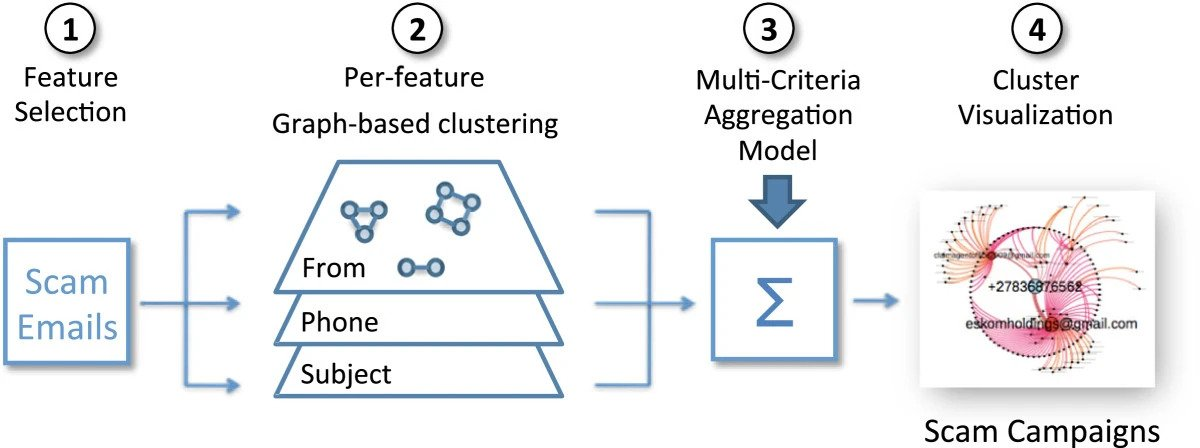
\includegraphics[scale=0.2]{slike/3.jpg}
\end{center}
\caption{‘TRIAGE’ workflow on scam dataset}
\label{fig:slika2}
\end{figure}

У трећем кораку, појединачне сличности карактеристика се агрегирају помоћу агрегатног модела који одражава понашање високог нивоа које је дефинисао аналитичар, који може одредити, на пример да је потребно најмање \emph{k} веома сличних особина (од \emph{n}) да бисмо узорке могли приписати истој кампањи. Омогућено је додељивање тежина тако да одређеним карактеристикама можемо бити дат већи или мањи значај. У табели \ref{tab:tabela3} приказан је скуп тежина коришћен на нашем скупу података, у којем је наглашен значај телефонских бројева и тема е-поште. Особинама везаним за е-адресе пошиљаоца дат је средњи значај, док је датуму слања дат мали значај. Укупна добијена вредност (агрегирана вредност) се потом користи као улаз за класичнe \emph{graph clustering} алгоритме, попут \emph{minimal cut} и \emph{connected components} који нам могу дати кластере произвољне величине и облика.

\begin{table}[h!]
\begin{center}
\caption{Weights of individual features (total = 1)}
\begin{tabular}{|c|c|} \hline
\textbf{Feature} & \textbf{Importance} \\ \hline
Phone & 0.30\\ \hline
From & 0.12\\ \hline
Reply & 0.18\\ \hline
Subject & 0.25\\ \hline
Email body & 0.1\\ \hline
Date & 0.05\\ \hline
\end{tabular}
\label{tab:tabela3}
\end{center}
\end{table}

У овој фази, важно је нагласити да се, осим можда телефонског броја који користи нападач (осим ако је овај број лажан), ниједна друга особина укључена у анализу не може сматрати сама по себи деовољном за приписивање \emph{скам} порука истом нападачу. На пример, чињеница да је иста (или слична) адреса е-поште пошиљаоца коришћена у две \emph{скам} поруке, чак и послате истог датума, не мора нужно значити да те две поруке потичу од истог појединца. Само једна или две заједничке карактеристике могу се појавити као последица случајности, или можда неке уобичајене технике коју нападачи деле. Ово мотивише избор фузионог модела са више критеријума који укључује различите тежине дефинисане према \emph{Regular Increasing Monotone - RIM} квантификатору \cite{rim}, што нам омогућава да моделирамо стратегије као што су - најмање \emph{k} јаких корелација је потребно за повезивање два мејла.

\subsection{Резултати кластеровања и експериментална валидација}
Алат за кластеровање \emph{'TRIAGE'} идентификовао је 1.040 кластера који се састоје од најмање 5 \emph{скам} порука повезаних различитим комбинацијама особина. Због начина генерисања ових кластера (тј. агрегације по више критеријума), очекујемо да ти кластери мејлова представљају различите кампање, које потенцијално могу организовати исти појединци - пошто мејлови у истом кластеру деле неколико заједничких особина.

Табела \ref{tab:tabela4} пружа неке глобалне статистике израчунате у 250 највећих \emph{скам} кампањи. У више од половине ових кампања преваранти користе само два различита телефонска броја, али и даље користе више од пет различитих поштанских сандучића како би добили одговоре од својих жртава. Већина кампања је прилично дуготрајна (у просеку траје око годину дана). Напомињемо да су величине кластера у просеку мале, што указује на то да постоји много малих, изолованих кампањи и да само неколико десетина порука припада истој кампањи. Ово би такође могла бити последица процеса прикупљања података; ипак, предвиђамо да би ово такође могло одражавати понашање \emph{скамера} који би можда желели да остану \emph{испод радара}. Заиста, велике количине истих порука е-поште имале би већи потенцијал да угрозе њихове \emph{скам} операције, јер би то постало видљиво за филтере нежељене поште засноване на садржају (енг.~{\em content-based filters}), па би бивали блокирани у ранијим фазама филтрирања е-поште. 


\begin{table}[h!]
\begin{center}
\caption{Global statistics of the top 250 clusters}
\begin{tabular}{|c|c|c|c|} \hline
\textbf{Statistic} & \textbf{Average} & \textbf{Median} & \textbf{Maximum} \\ \hline
Number of emails & 38 & 28 & 376\\ \hline
Number of from & 13.9 & 9 & 181\\ \hline
Number of replies & 6.2 & 5 & 56\\ \hline
Number of subjects & 9.9 & 7 & 114\\ \hline
Number of phones & 2.5 & 2 & 34\\ \hline
Duration (in days) & 396 & 340 & 1.454\\ \hline
Number od dates(distinct) & 27.9 & 22 & 259\\ \hline
Compactness & 2.5 & 2.4 & 5.0\\ \hline
\end{tabular}
\label{tab:tabela4}
\end{center}
\end{table}

\subsubsection{Процена резултата кластеровања}
Како је кластеровање података у основи приступ класификације без надзора, важно је проценити резултате груписања помоћу објективних критеријума, како би се потврдила ваљаност резултата. Постоје два приступа за вршење ове валидације: \textbf{екстерна} и \textbf{интерна} евалуација.

Да бисмо проценили квалитет наших резултата груписања, испитана је њихова укупнa компактност, разврстана по појединачним карактеристикама. Компактност графикона је индекс ваљаности кластера који показује колико су кластери \emph{компактни} (или хомогени), на основу њихових карактеристика унутар повезивања. Компактност одражава просечну сличност ивица између два објекта кластера.

Пошто алат \emph{'TRIAGE'} прати све појединачне везе у графиконима сличности, такође је могуће израчунати удео порука е-поште које су повезане посебним комбинацијама особина унутар кластера. Ово може бити веома корисно за разумевање разлога за формирање кластера и на тај начин пружити увид у \emph{стабилне} (мање променљиве) карактеристике које користе преваранти приликом извођења нових кампања.

У табели \ref{tab:tabela5} можемо приметити да најчешћа комбинација која повезује \emph{скам} поруке (у 13\% случајева) укључује телефонски број, тему, као и све три адресе е-поште (пошиљалац, одговор, тело мејла). Да бисмо потврдили интуицију о важности одређених карактеристика (телефонских бројева, и у мањој мери, адреса е-поште) и њиховој ефективној улози у идентификовању кампањи, разматрамо све везе засноване на сличности унутар кластера. Уочавамо да особине које су углавном одговорне за повезивање \emph{скам} порука у кластерима укључују телефонске бројеве (у 88\% случајева), затим адресу е-поште одговора (за 66\% веза). Није изненађујуће што се адреса пошиљаоца (која се лако може лажирати) мења много чешће и користи се као повезујућа карактеристика у само 46\% случајева.

\begin{table}[h!]
\begin{center}
\caption{Top coalitions of features across all clusters}
\begin{tabular}{|c|c|c|c|} \hline
\textbf{Coalition} & \textbf{Percentage (\%)}\\ \hline
(phone, subject, from, reply, email body) & 13\\ \hline
(phone, reply, email body) & 12\\ \hline
(phone, subject, reply, email body) & 11\\ \hline
(phone, from, reply, email body) & 7\\ \hline
(phone, subject) & 6\\ \hline
(phone, from) & 5\\ \hline
(phone, reply) & 4\\ \hline
(phone, reply, subject) & 4\\ \hline
(phone, reply, subject, from) & 4\\ \hline
others & 33\\ \hline
\end{tabular}
\label{tab:tabela5}
\end{center}
\end{table}

\section{\emph{Макро-кластери}: повезивање поткампањи}
У следећем кораку смо \emph{скам} кампање посматрали из шире перспективе: тражењем слабо повезаних кластера. Циљ је био да се укаже на могуће кампање већег обима, које су сачињене од међусобно слабо повезаних \emph{скам} операција (тј. различитих превара). У ту сврху користили смо само адресе е-поште и телефонске бројеве, будући да се други атрибути не сматрају подацима за личну идентификацију. У ствари, тражили смо кластере који деле најмање једну адресу е-поште и/или телефонски број и користили те информације за изградњу такозваних \emph{макро-кластера}.

Као резултат тога, идентификовали смо скуп од 845 изолованих кластера и други скуп од 195 повезаних кластера, при чему се потоњи састоји од 62 \emph{макро-кластера}. Карактеристике првих шест макро кампања приказане су у табели \ref{tab:tabela6}. Ови \emph{макро-кластери} су посебно занимљиви јер се састоје од скупа \emph{скам} кампањи које су слабо повезане и стога могу бити организоване од стране истих сајбер криминалаца. Заправо, везе између различитих кластера алгоритам за груписање је сматрао преслабим, због шеме одлучивања и прагова постављених за параметре, па су стога ти \emph{скамови} на крају груписани у засебне кластере. Међутим, ове слабе везе се лако могу повратити, а на аналитичару је да истражи колико су те међусобне везе заиста значајне. Заиста, сајбер истражитељу много је лакше да почне од скупа заиста смислених кластера, а затим да постепено повећава прагове до тачке у којој може сам одлучити да престане са спајањем група података, јер више нема смисла приписивати различите кампање истој групи због недостатка доказа.

\begin{table}[h!]
\tiny
\begin{center}
\caption{Macro-cluster, mean values of attributes}
\hspace*{-6em}
\begin{tabular}{|c|c|c|c|c|c|c|l|} \hline
\textbf{Number} & \textbf{Number of campaigns} & \textbf{Phones} & \textbf{Mailboxes} & \textbf{Subjects} & \textbf{Duration (years)} & \textbf{Countries} & \textbf{Topics}\\ \hline
1 & 14 & 44 & 677 & 223 & 4 & 4 & Lottery, lost funds, investments\\ \hline
2 & 43 & 163 & 1.127 & 463 & 4 & 7 & Lottery, banks, diplomats, FBI\\ \hline
3 & 6 & 18 & 128 & 80 & 4 & 4 & Lottery\\ \hline
4 & 5 & 8 & 111 & 51 & 3.5 & 2 & Packaging, lottery, loans\\ \hline
5 & 6 & 7 & 201 & 96 & 1 & 1 & Lottery, UPS \& WU delivery\\ \hline
6 & 4 & 7 & 82 & 33 & 2 & 1 & Diplomats, monetary and payments scam\\ \hline
\end{tabular}
\label{tab:tabela6}
\end{center}
\end{table}

\section{Закључак}

У овом раду анализирана је студија француских истраживача у којој је емпиријски показано постојање 419 преваре и кључна улога коју телефонски бројеви и адресе е-поште имају у овим преварама, за разлику од других шема сајбер криминала у којима се адресе е-поште често могу лажирати, а телефонски бројеви ретко користити. Помоћу технике вишедимензионалног кластеровања идентификовано је на посматраном скупу података око 1.000 \emph{скам} кампањи.

Приказани су начини на које се кластери издвајају и њихове опште статистике. На крају, указано је на методе које нам омогућују откривање постојање слабих веза између наизглед неповезаних сајбер превара које чине макрокампање за које са великом вероватноћом можемо тврдити да су вођене од стране истих сајбер-криминалаца. Утврђено је да су неке од ових макро-кампањи географски распоређене у неколико земаља, афричких и европских. Анализа је открила велику разноликост у начину увлачења жртве у превару, као и у вођењу кампање. Међу \emph{скамерима} постоји велика конкуренција у актуелности тема преваре.





 

\addcontentsline{toc}{section}{Литература}
\appendix

\iffalse
\bibliography{seminarski} 
\bibliographystyle{plain}
\fi

\begin{thebibliography}{9}

\bibitem{article} Isacenkova, Jelena, et al. "Inside the scam jungle: A closer look at 419 scam email operations." EURASIP Journal on Information Security 2014.1 (2014): 1-18.

\bibitem{def} Definition of Nigerian Scam, http://www.419scam.org/419scam.htm

\bibitem{prosecuting} Buchanan J, Grant AJ: Investigating and prosecuting Nigerian Fraud. United States Attorneys’ Bulletin 2001., 49(6):

\bibitem{org} 419 Scam - fake lottery Fraud phone directory, http://www.419scam.org/419-by-phone.htm

\bibitem{phone} Costin A, Isacenkova J, Balduzzi M, Francillon A, Balzarotti D: The role of phone numbers in understanding cyber-crime. In 11th International Conference on Privacy, Security and Trust (PST 2013). Tarragona, Catalonia; 10-12 July, 2013.

\bibitem{study} Pathak A, Qian F, Hu YC, Mao ZM, Ranjan S: Botnet spam campaigns can be long lasting: evidence, implications, and analysis. In SIGMETRICS ’09 Proceedings of the Eleventh International Joint Conference on Measurement and Modeling of Computer Systems Seattle, WA, 15-19 June. New York: ACM; 2009:13-24.

\bibitem{cishi} Anderson DS, Fleizach C, Savage S, Voelker GM: Spamscatter: Characterizing internet scam hosting infrastructure. PhD thesis, University of California, San Diego 2007

\bibitem{microsoft} Microsoft Security Intelligence Report (2008-2012), http://www.microsoft.com/security/sir/archive/default.aspx

\bibitem{botnet} Thonnard O, Dacier M: A strategic analysis of spam botnets operations. In Proceedings of the 8th Annual Collaboration, Electronic messaging, Anti-Abuse and Spam Conference, CEAS ’11. New York: ACM; 2011:162-171.

\bibitem{target} Thonnard O, Bilge L, O’Gorman G, Kiernan S, Lee M: Industrial espionage and targeted attacks: understanding the characteristics of an escalating threat. In RAID, Amsterdam, The Netherlands, 12-14 September. New York: Springer; 2012:64-85.

\bibitem{rogueav} Cova M, Leita C, Thonnard O, Keromytis AD, Dacier M: An analysis of rogue AV campaigns. In Proceedings of the 13th International Conference on Recent Advances in Intrusion Detection. RAID’10, Berlin, Heidelberg: Springer-Verlag; 2010:442-463. [http://portal.acm.org/citation.cfm?id=1894166.1894196]

\bibitem{triage} Thonnard O: A multi-criteria clustering approach to support attack attribution in cyberspace. PhD thesis, École Doctorale d’Informatique, Télécommunications et Électronique de Paris, 2010

\bibitem{ngram} Kondrak G: N-gram similarity and distance. In Proceedings of the 12th Conference on String Processing and Information Retrieval Buenos Aires,2–4November. Heidelberg: Springer-Verlag Berlin; 2005:115-126. 

\bibitem{rim} Zadeh LA: A computational approach to fuzzy quantifiers in natural languages. Comput. \& Math. Appl 1983, 9: 149-184.


\end{thebibliography}

\end{document}
